\documentclass[fleqn, 12pt]{extarticle}
\usepackage{textbook}
\input{vc.tex}

\begin{document}
\selectlanguage{russian}

\title{\textbf{Организация Станций Страховки}\\
\large{Краткое Справочное Пособие}}
\author{\textsc{Юлия Беляева}\\\textit{а/к Политехник}}
\date{\GITAuthorDate}

\maketitle

\begin{abstract}
	Данное справочное пособие -- это дополнение к лекциям и тренировкам, проводимым в альпклубе <<Политехник>>. Оно описывает некоторые принципы и техники организации станций,
	оставляя за рамками многие вещи, которые разбираются на тренировках и практических занятиях. Использование данного материала для самостоятельного изучения темы с нуля без инструктора не
	рекомендуется.
\end{abstract}

\section{Что такое станция}
Станцией называется пункт прикрепления к рельефу (скале, льду и т.п.) используемый альпинистами для взаимостраховки и самостраховки, для
закрепления перил и дюльферов и т.п. Данный текст рассказывает про станции страховки, далее для краткости просто <<станции>>. Типичная станция состоит из одной или нескольких точек,
объединённых (сблокированных) между собой репшнуром или стропой (см. список материалов в разд.~\ref{sec:advice}). Пункт используемый для организации страховки и
самостраховки называют центральным пунктом станции.
Чаще всего центральный пункт станции -- это муфтованный карабин, называемый мастер-карабином или станционным карабином.

\section{Что такое <<хорошая станция>>}
	Есть четыре основных требования предъявляемых к станциям:
    \begin{itemize}
        \item \textbf{Надёжность.} Станция должна выдерживать всевозможные нагрузки, которые могут на неё прийтись: статические нагрузки, создаваемые висящими на станции людьми
                и снаряжением, и динамические нагрузки, вызванные срывами. Наиболее опасен срыв лидера сразу после станции до постановки первой точки (срыв с фактором близким к двум),
                так как нагрузка на станцию в этот момент наибольшая. Надёжность станции прежде всего зависит от надёжности точек, на которых она основана.
        \item \textbf{Дублирование} означает, прежде всего, использование нескольких точек для организации станции, чтобы предотвратить её разрушение в случае отказа одной из точек. 
                Кроме того, часто дублируют петли, в особенности, если есть опасность их попадания на острую скальную кромку. Также понятие дублирования включает в себя использование 
                для станции нескольких разных элементов рельефа, например, вместо того чтобы располагать все точки в одной и той же щели.
        \item \textbf{Равномерное распределение нагрузки} означает, что нагрузка, действующая на станцию, не приходится целиком на одну из точек, а распределяется между ними. 
                Это уменьшает риск отказа точек. Важно помнить, что нагрузка действующая на станцию не обязательно направлена вертикально вниз, она может быть направлена как 
                и под небольшим углом к вертикали, так и сильно в сторону. Кроме того при срыве лидера рывок на станцию может быть направлен вверх. Возможные направления рывка 
                нужно учитывать при организации станции.
        \item \textbf{Отсутствие проседания} означает, что при отказе одной из точек станция не должна сильно проседать, создавая динамическую нагрузку на оставшиеся точки.
    \end{itemize}
    
    Важно понимать, что:
    \begin{itemize}
        \item эти четыре требования не являются исчерпывающими, это просто хорошая практика организации станций;
        \item невозможно удовлетворить этим требованиям на сто процентов, нужно удовлетворить им достаточно хорошо для данной ситуации, затратив не слишком много времени и снаряжения; 
              при этом станция должна оставаться как можно более простой;
        \item требования <<равномерное распределение нагрузки>> и <<отсутствие проседания>> конфликтуют между собой, в зависимости от ситуации отдаётся приоритет одному из них.
    \end{itemize}

\subsection{Надёжные точки}
    Самое важное в организации надёжной станции -- это постановка надёжных точек. Если есть несколько хороших точек, то выбор способа их блокировки в станцию -- дело техники.
    Пытаться хитроумными способами блокировать плохие точки не нужно, такая станция получится опасной. Лучше просто поискать другие места под точки.

    Надёжность точек прежде всего зависит от:
    \begin{itemize}
        \item состояния скалы в которой стоит точка: хрупкости и мягкости породы, разрушенности скалы, обледенения и т.п.;
        \item качества собственно постановки, т.е. правильности выбранного вида, формы и размера закладного элемента, качества его расположения в скале и
              того насколько хорошо он <<заклинен>>, и других специфичных для конкретных видов закладных элементов факторов;
        \item размера закладного элемента (чем больше тем надёжней);
        \item соответствия направления в котором лучше всего работает точка и направления нагрузки на неё в станции.
    \end{itemize}

\section{Станции на одной точке}
    Станции на одной точке организуют на естественных элементах рельефа: деревьях, больших валунах, скальных выступах, отколах. Важно убедиться в абсолютной надёжности единственной точки. 
    Шлямбура, закладки, крючья, ледобуры и т.п. не считаются достаточно надёжными для использования как единственная точка станции.

   	При организации станции на дереве важно проверить что:
    \begin{itemize}
        \item дерево живое, не сухое и неповреждённое;
        \item оно достаточно большое;
        \item оно хорошо сидит в почве (для проверки лидер трясёт дерево руками).
    \end{itemize}
    
    \begin{figure}
        \centering
        \begin{minipage}[t]{0.45\textwidth}
            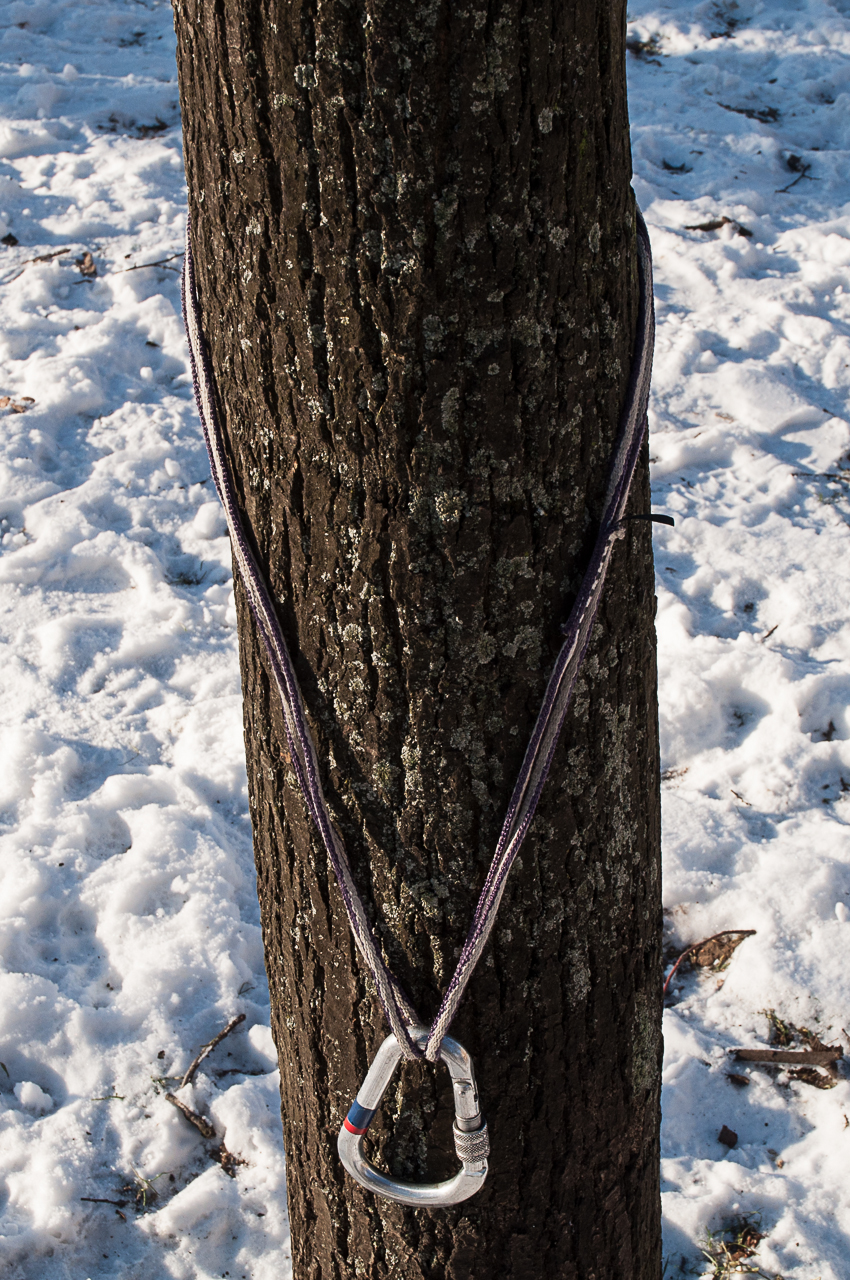
\includegraphics[width=\textwidth]{tree1}
            \captionof{figure}{Простейший вариант станции на дереве.}\label{fig:tree1}
        \end{minipage}\hspace{0.05\textwidth}
        \begin{minipage}[t]{0.45\textwidth}
            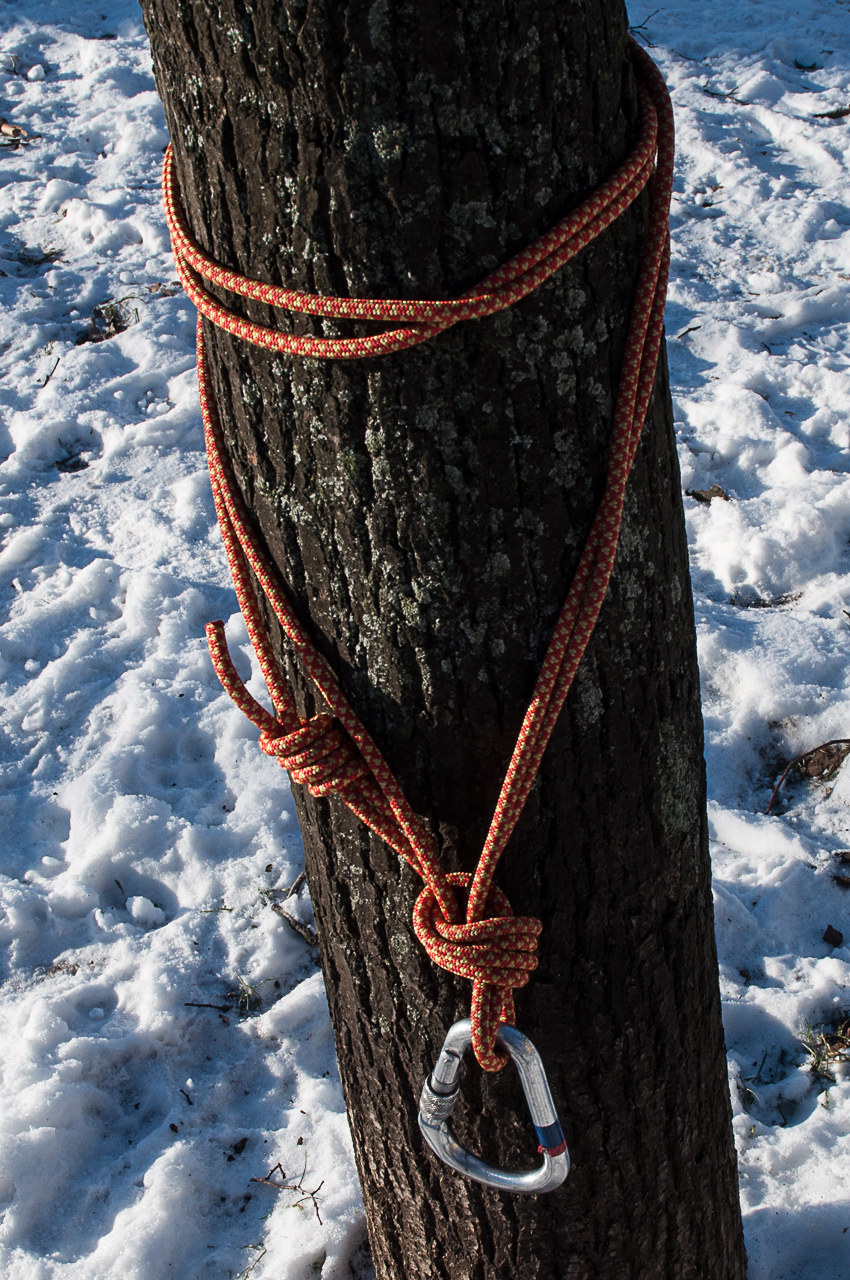
\includegraphics[width=\textwidth]{tree2}
            \captionof{figure}{Улучшенный вариант станции с центральным узлом и дополнительным оборотом вокруг ствола дерева.}\label{fig:tree2}
        \end{minipage}
    \end{figure}

	Простейшая станция на дереве организуется оборачиванием петли вокруг ствола (рис.~\ref{fig:tree1}). В два конца петли вставляется карабин, который играет роль центрального пункта станции.
    Важно чтобы угол между двумя концами петли, в которые продет станционный карабин, был острым
    (см. разд.~\ref{sec:multipoint.anchors}). При достаточной длине петли на ней завязывают узел восьмёрка или проводник. Он фиксирует правильное положение станционного карабина
    и исключает его нагрузку по трём направлениям. Образовавшаяся петля узла уже может играть 
    роль центрального пункта, это бывает удобно и экономит муфтованный карабин. Кроме того, станция оказывается более защищённой от перетирания стропы: для разрушения станции необходимо
    перерезать два оборота стропы, а не один. Дополнительный оборот петли вокруг ствола (если петля достаточно длинная)
    фиксирует положение станции на дереве (рис.~\ref{fig:tree2}).
    Запрещается использование узла удавка для этих целей, так как он сильно ослабляет стропу.
    Не рекомендуется делать станцию высоко на стволе дерева из-за образующегоcя рычага.

    Особенности использования элементов скального рельефа в качестве единственной точки станции:
    \begin{itemize}
        \item используемый элемент рельефа должен быть большим;
        \item валуны держатся на месте не только за счёт своего веса, но и за счёт расположения, важно проверить что используемый валун не сдвинется с места;
        \item выступы и отколы должны быть хорошо соединены с основной скалой;
        \item нужно подвигать, покачать используемый выступ, откол или камень, он должен быть абсолютно неподвижен;
        \item нужно постучать по скале молотком и убедиться что она издаёт звонкий звук;
        \item скалы не должны иметь острые края, которые могли бы перерезать петлю/репшнур;
        \item форма выступа не должна позволять петле с него соскочить.
    \end{itemize}
    
    Полезно придерживаться этих же рекомендаций при использовании элементов рельефа как промежуточных точек страховки.
    \begin{figure}[h]
        \centering
        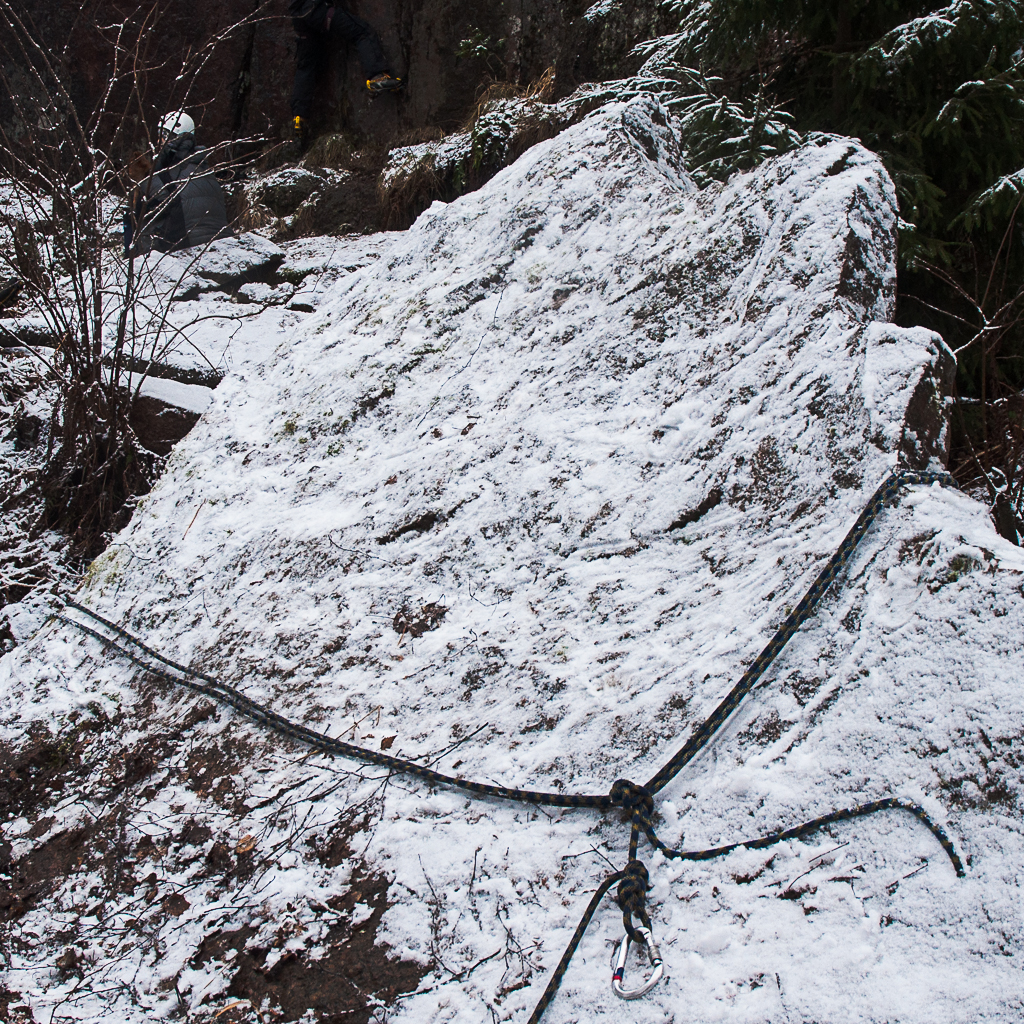
\includegraphics[width=0.45\textwidth]{bowline}
        \caption{Станция на выступе из основной верёвки, завязанной двойным булинём.}\label{fig:bowline}
    \end{figure}
    
    Станции на рельефе организуются оборачиванием или набрасыванием петли на элемент рельефа аналогично станциям на дереве. Кроме петель из стропы или репшнура можно использовать
    связочную верёвку, завязав на конце двойной булинь (рис.~\ref{fig:bowline}). Также для организации станций можно использовать песочные часы -- сквозные отверстия в скале --
    или пробки -- заклинившие в каминах или расщелинах обломки скалы, продевая через них петлю или репшнур.

\section{Станции на нескольких точках}\label{sec:multipoint.anchors}
    Существует множество способов блокировки нескольких точек в станцию. В наиболее распространённых методах точки блокируются друг с другом
    так, что центральный пункт станции соединён с каждой точкой отдельной ветвью из репшнура или стропы. При этом нагрузка на центральный пункт распределяется между ветвями.
    Распределение сил в станции зависит от направления приложенной силы и угла между ветвями станции
    (табл.~\ref{tab:angle}). Для некоторых способов блокировки (например, для станции с фиксированным центральным узлом, разд.~\ref{sec:cordelette}) оно так же зависит от разницы длин ветвей.
    \begin{table}[h]
        \centering
        \begin{tabular}{|c|c|}
            \hline
            \multirow{2}{*}{угол между ветвями станции} & процент от общей нагрузки \\ & приходящийся на каждую точку \\
            \hline
            $30^o$ & $52\%$ \\
            $45^o$ & $54\%$ \\
            $60^o$ & $58\%$ \\
            $90^o$ & $71\%$ \\
            $120^o$ & $100\%$ \\
            $150^o$ & $193\%$ \\
            $170^o$ & $574\%$ \\
            \hline
        \end{tabular}
        \caption{Распределение нагрузки между двумя точками станции в зависимости от угла между её ветвями.}\label{tab:angle}
    \end{table}
    
    Изменение направления нагрузки по-разному влияет на её распределение между точками в зависимости от выбранной схемы блокировки. Схемы которые при изменении направления
    действующей силы перестраиваются и продолжают грузить точки с одинаковой силой, называются схемами с динамическим (или автоматическим) распределением, а процесс перестройки 
    называется компенсацией. Минусом компенсации является наличие некоторого количества слабины в системе, из-за которой при отказе одной из точек происходит проседание станции. 
    Схемы с жёсткой блокировкой точек, не допускающей перестройку, называются схемами со статическим распределением нагрузки. Минус таких схем, кроме отсутствия компенсации,
    в том что при разной длине ветвей станции при рывке короткая ветвь нагружена больше, чем длинная.
    
    Компенсация в станции нужна:
    \begin{itemize}
        \item при изменении направления движения;
        \item при возможности маятника при срыве на траверсе;
        \item если станция находится на полке, где участники могут перемещаться;
        \item если станцию использует большая группа людей которые нагружают её в разных направлениях.
    \end{itemize}

\subsection{Компенсационная петля и её варианты}
    Компенсационная петля является схемой с динамическим распределением нагрузки.
    
    \subsubsection{Компенсационная петля на двух точках}
    \begin{figure}[h]
        \centering
        \begin{minipage}[t]{0.45\textwidth}
            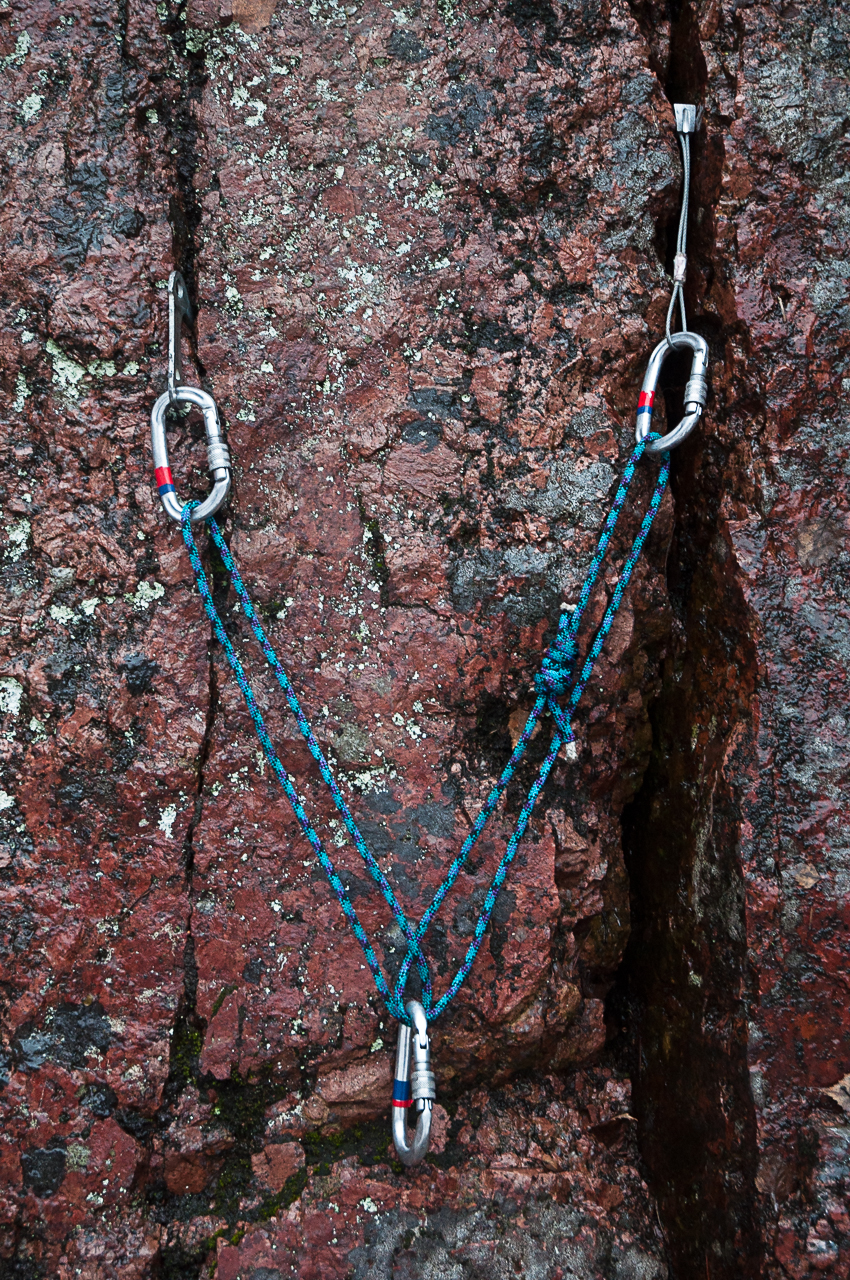
\includegraphics[width=\textwidth]{slidx2}
            \captionof{figure}{Классическая компенсационная петля на двух точках.}\label{fig:slidx2}
        \end{minipage}\hspace{0.05\textwidth}
        \begin{minipage}[t]{0.45\textwidth}
            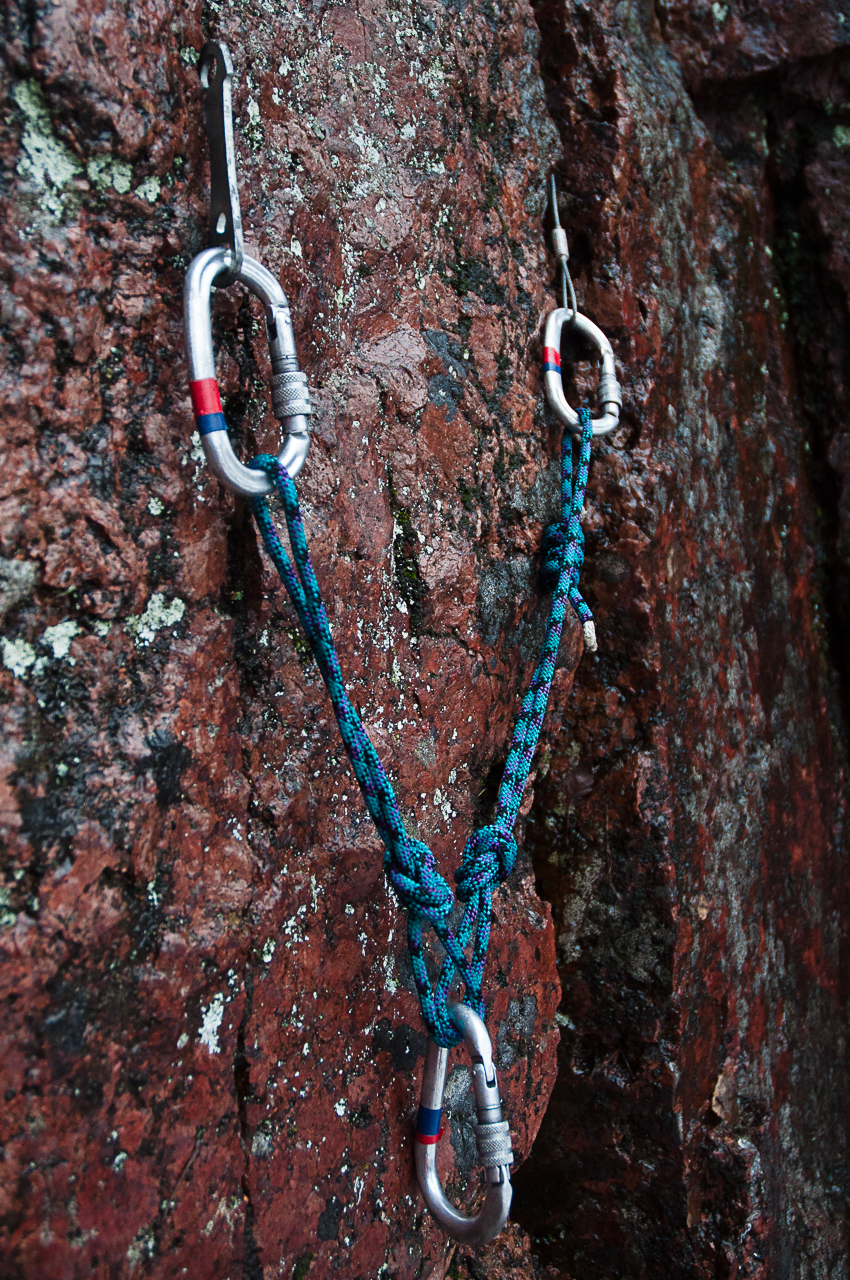
\includegraphics[width=\textwidth]{slidx2_knots}
            \captionof{figure}{Компенсационная петля с узлами-ограничителями на двух точках.}\label{fig:slidx2_knots}
        \end{minipage}
    \end{figure}
    
    Станция на основе компенсационной петли (рис.~\ref{fig:slidx2}) организуется следующим образом: петля вщёлкивается в карабины в точках; ветви петли соединяются друг с другом;
    при этом на одной из ветвей делается перекрут (рис.~\ref{fig:slidx2_details}). В этот перекрут вставляется карабин который одновременно вщёлкивается в другую ветвь.
    Благодаря такой структуре станция не разваливается при отказе одной из точек. 
    
    В такой схеме станционный карабин свободно перемещается по петле, поэтому станция хорошо распределяет
    нагрузки между точками в широком диапазоне направлений.
    Способность карабина перемещаться зависит от трения в петле. Поэтому компенсационная петля хорошо работает с тонкими дайнимовыми стропами или репшнуром и хуже
    с толстыми нейлоновыми стропами. Чтобы сшивка петли (или узел на репшнуре) не мешали станционному карабину скользить по петле, лучше располагать их ближе к одной из точек.
    На станции с разными длинами плеч сшивка (узел) должна находиться на коротком плече, чтобы не попасть в станционный карабин при возможном перевороте станции.
    
	Главный недостаток компенсационной петли это сильное проседание станции при отказе одной из точек, которое приводит к большой динамической нагрузке на оставшуюся точку.
    Поэтому такая станция может быть опасной на потенциально слабых точках. Кроме того, в данной схеме отсутствует дублирование в петле. Это значит, что при разрыве петли, например
    при попадании на острую скальную кромку, станция полностью разрушается.
    
    Завязывание узлов-ограничителей (проводник или восьмёрка, рис.~\ref{fig:slidx2_knots}) позволяет сократить возможное проседание станции до приемлемого (за счёт уменьшения степени компенсации)
    и обеспечивает дублирование петли. Кроме того, при вылете одной из точек ограничитель немного проскользнёт
    и частично компенсирует рывок, что ещё более уменьшит нагрузку на оставшуюся точку.
    Расстояние между ограничителями должно быть не больше 40-60см (допустимо не вязать узлы на петлях длиной меньше 60см).
    При организации станции рекомендуется оценить требуемую степень компенсации и завязать узлы как можно ближе друг к другу.
    
    \begin{figure}
        \centering
        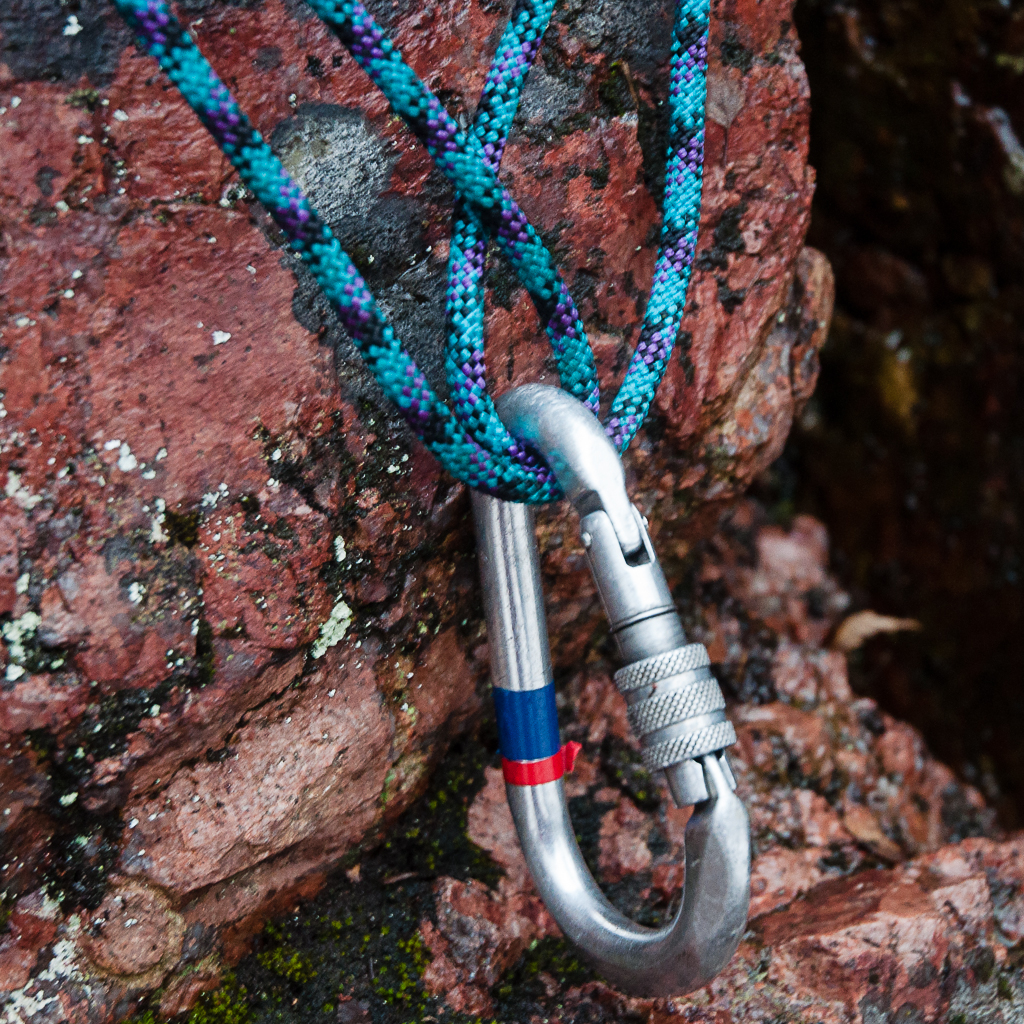
\includegraphics[width=0.45\textwidth]{slidx2_details}
        \caption{Центральный пункт в классической компенсационной петле крупным планом.}\label{fig:slidx2_details}
    \end{figure}
    
    \subsubsection{Компенсационная петля на трёх точках}
    Если в станции на трёх точках нужна компенсация то используют компенсационную петлю со стременами.
    \begin{figure}[h]
        \centering
        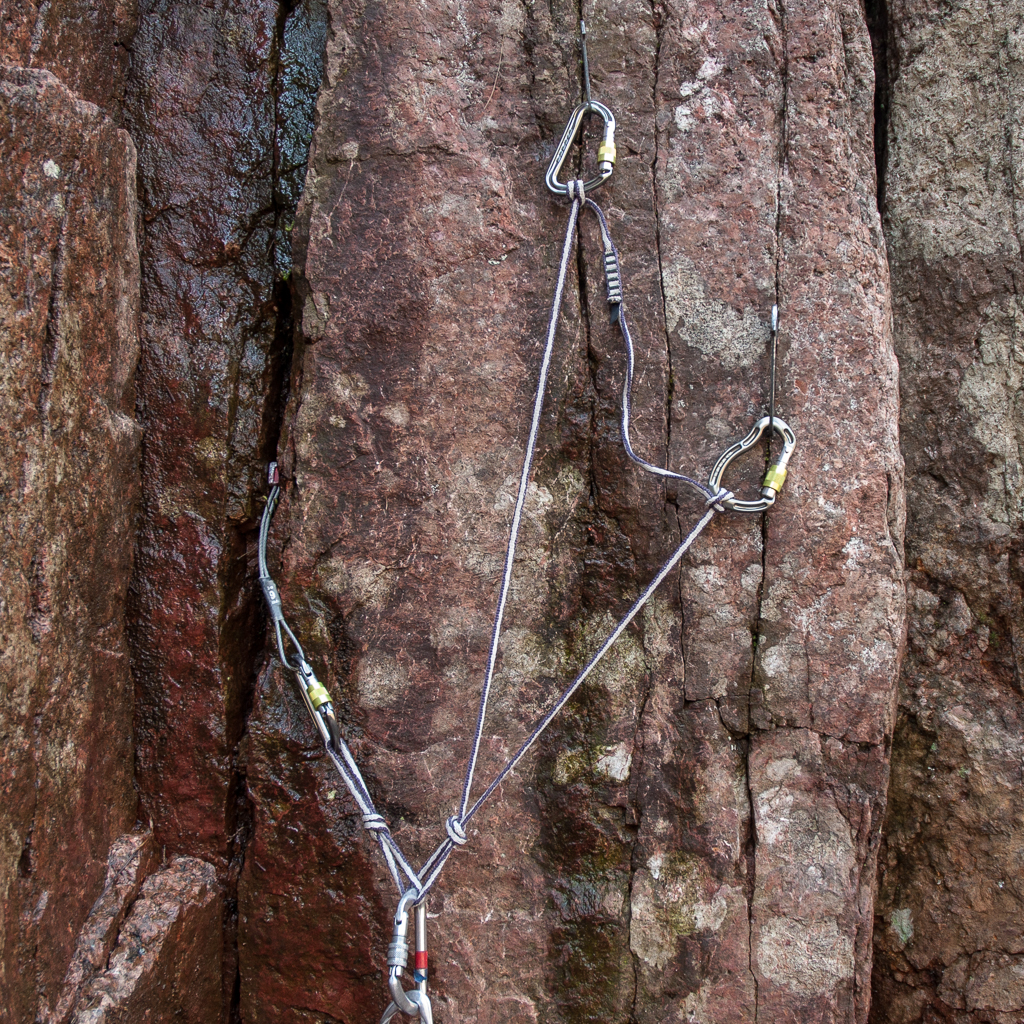
\includegraphics[width=0.45\textwidth]{slidx3_clove}
        \caption{Компенсационная петля на трёх точках со стременами.}\label{fig:slidx3_clove}
    \end{figure}
    Компенсационная петля на трёх точках со стременами (рис.~\ref{fig:slidx3_clove}) организуется следующим образом. Выбираются две соседние близко расположенные точки. Они составят
    одну ветвь станции. На эти точки вешается петля и закрепляется на них стременами таким образом чтобы участок петли между точками не был натянут. Второй конец петли вешается на другую точку.
    Это вторая ветвь станции. Далее на каждой ветви завязывают узлы-ограничители. Сначала отмеряется положение узла на ветви со стременами. Затем, после завязывания
    первого узла определяется положение другого узла. После завязывания ограничителей между ними делается перекрут, такой же как и в компенсационной петле на двух точках, в него и в другую
    ветвь петли вщёлкивается мастер-карабин. В целом станция получается похожей на компенсационную петлю на двух точках с ограничителями, с той разницей что одна из ветвей станции
    закреплена одновременно на двух точках.
    
    Такая станция компенсирует изменение направления нагрузки так же хорошо,
    как и компенсационная петля на двух точках: на каждую из ветвей станции приходится приблизительно половина нагрузки. Однако в ветви со стременами нагрузка уже не
    распределена равномерно, так как точки со стременами соединены фиксированной связью. Из-за этого важно при организации такой станции подобрать правильные
    положения стремян на точках.

\subsection{Станция с фиксированным центральным узлом}\label{sec:cordelette}
    Станция с фиксированным центральным узлом это схема со статическим распределением нагрузки.

    \subsubsection{Станция с фиксированным центральным узлом на двух и трёх точках}
    \begin{figure}[h]
        \centering
        \begin{minipage}[t]{0.45\textwidth}
            \centering
            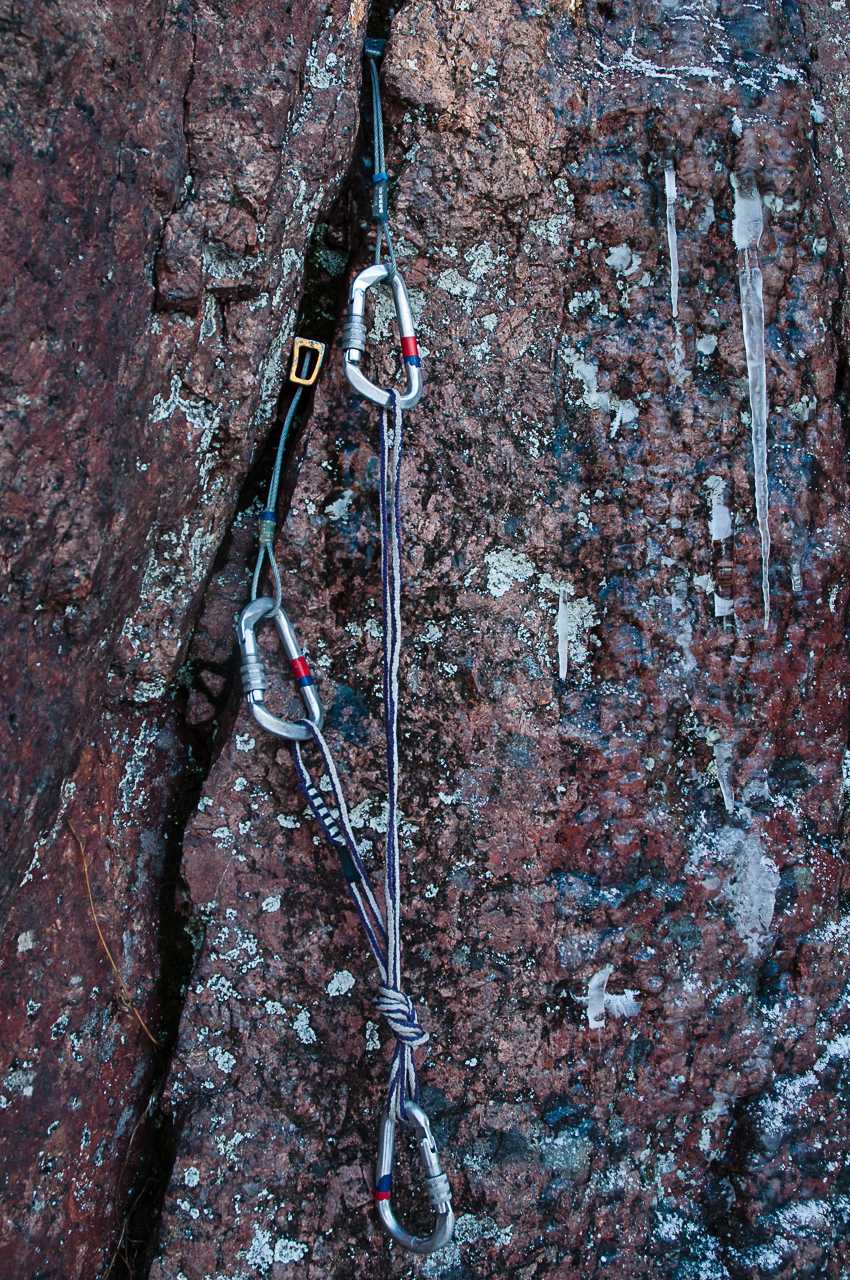
\includegraphics[width=\textwidth]{cordelette2}
            \captionof{figure}{Станция с фиксированным центральным узлом на двух точках.}\label{fig:cordelette2}
        \end{minipage}\hspace{0.05\textwidth} 
        \begin{minipage}[t]{0.45\textwidth}
            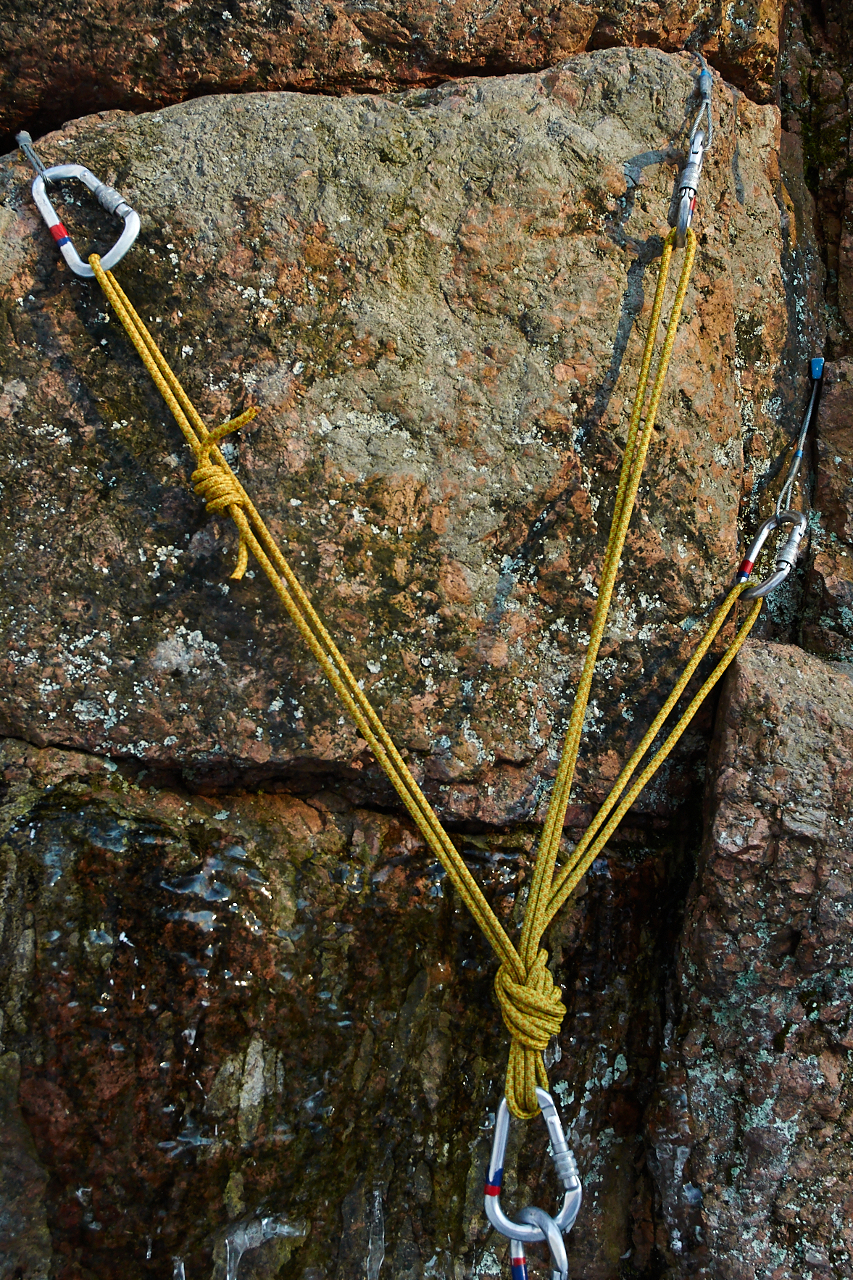
\includegraphics[width=\textwidth]{cordelette3}
            \captionof{figure}{Станция с фиксированным центральным узлом на трёх точках.}\label{fig:cordelette3}
        \end{minipage}
    \end{figure}
    Для организации станции с фиксированным центральным узлом надо: определить направление ожидаемой нагрузки; вщёлкнуть петлю в карабины в точках и натянуть в этом направлении;
    завязать восьмёрку или проводник для получения независимых ветвей (рис.~\ref{fig:cordelette2}).
    Станция с фиксированным центральным узлом на трёх точках делается аналогично (рис.~\ref{fig:cordelette3}).
    Для того чтобы узел легче было развязать после нагружения станции,
    в узел вставляют карабин (не нарушая целостности его структуры). Получившуюся петлю можно использовать в качестве центрального пункта станции.
    
    Нагрузка в станции с фиксированным центральным узлом распределяется равномерно между точками только если она направлена определённым образом,
    поэтому очень важна правильная настройка положения центрального узла. Если направление нагрузки меняется, то одна или несколько ветвей станции оказываются ненатянутыми и вся нагрузка приходится
    только на одну точку. Силы в станции также распределяются неравномерно если длины плеч станции с фиксированным центральным узлом не равны.
    Например, такое происходит, если все точки станции находятся в одной вертикальной щели.
    В такой конфигурации при рывке большая часть нагрузки придётся на короткую ветвь.
    
    Большой плюс станции с фиксированным центральным узлом -- отсутствие проседания при отказе одной из точек. Кроме того, станция с фиксированным центральным узлом
    быстро и просто организуется.

\section{Процесс организации станции}
    Место для станции должно быть безопасным, т.е. по возможности защищённым от камнепадов и т.п., и удобным для нахождения там страхующего. Часто для станций лидер выберает полки.
    
    Наиболее удобно разместить станцию так, чтобы мастер карабин оказывался приблизительно на уровне солнечного сплетения человека. Для того чтобы сделать
    станцию выше, точки нужно будет поставить так высоко, что стоя на полке этого сделать уже не получится. Это неудобно как и для первого, который организовывает станцию,
    так и для последнего, который будет её разбирать. Если же станцию расположить ниже, то человек стоящий на полке не сможет подгрузить станцию своей самостраховкой.
    В таком случае срыв будет означать дополнительную динамическую нагрузку на точки станции, что нежелательно.
    
    Для того чтобы мастер карабин станции находился на удобной высоте, точки станции нужно расположить в зоне которую лидер может охватить руками. Таким образом,
    для того чтобы проверить подходит ли место для организации станции, нужно проверить что на этом участке рельефа есть возможность поставить несколько надёжных точек.
    Если поставить хорошие точки представляется сложным, стоит поискать другое место для станции.

    После выбора места лидер ставит несколько надёжных точек, не думая пока о способе их блокировки. Когда точки поставлены, лидер блокирует их в станцию.

\section{Технические рекомендации}\label{sec:advice}
    При организации станций полезно придерживаться следующих рекомендаций:
    \begin{itemize}
        \item Для точек станции рекомендуется использовать самые большие из имеющихся подходящих по размеру закладных элементов:
              самые большие гексы, самые большие закладки, самые большие камалоты.
        \item Мастер-карабин -- муфтованный, замуфтовывается при организации станции первым участником и размуфтовывается только при разбирании станции последним участником.
        \item Все карабины должны быть по возможности развёрнуты <<муфтой от скалы>>.
        \item Для блокировки точек в многоточечных станциях можно использовать:
            \begin{itemize}
                \item сшитые петли из стропы из нейлона или дайнимы/спектры;
                \item петли из нейлоновой стропы связанные ленточным узлом (встречный проводник);
                \item нейлоновый репшнур 7мм связанный узлом грейпвайн;
                \item репшнур из высокопрочного материала (кевлар, дайнима/спектра и т.п.) связанный узлом грейпвайн в три оборота;
                \item основную верёвку.
            \end{itemize}
        \item Для удлинения петель рекомендуется использовать карабины, вместо пропускания петли в петлю. Использование узла удавка (он же полусхватывающий узел) запрещено.
        \item Сшивка/узел в петле не должны попадать в узлы станции и карабины и не должны мешать компенсации в станциях с динамическим распределением нагрузки.
        \item Угол между ветвями станции не должен превышать $60^o$ для станций на двух точках и $90^o$ для станций на трёх точках.
    \end{itemize}
    
\nocite{*}
\bibliographystyle{plain}
\bibliography{anchors}
\end{document}
